
\chapter{Обсуждение Результатов}\label{chapt_results}
В результате полугода работы прибора ДЭПРОН накоплен большой массив информации - 35 тысяч файлов бинарных данных, общим объемом 141 МБайт. Эти данные являются сжатыми и после распаковки в человеко-читаемый табличный вид представлены массивом файлов объемом 1,3 Гб, эти данные собраны в файлы по дням года и осуществлена привязка данных к географическим и геомагнитным координатам.



Далее информация прибора ДЭПРОН была визуализирована с помошью пакета \texttt{lattice} и базовой графической системы R. На рисунке \ref{fig:depronseclog08-29-16} показаны результаты визуализации.
\begin{figure}[h]
	\centering
	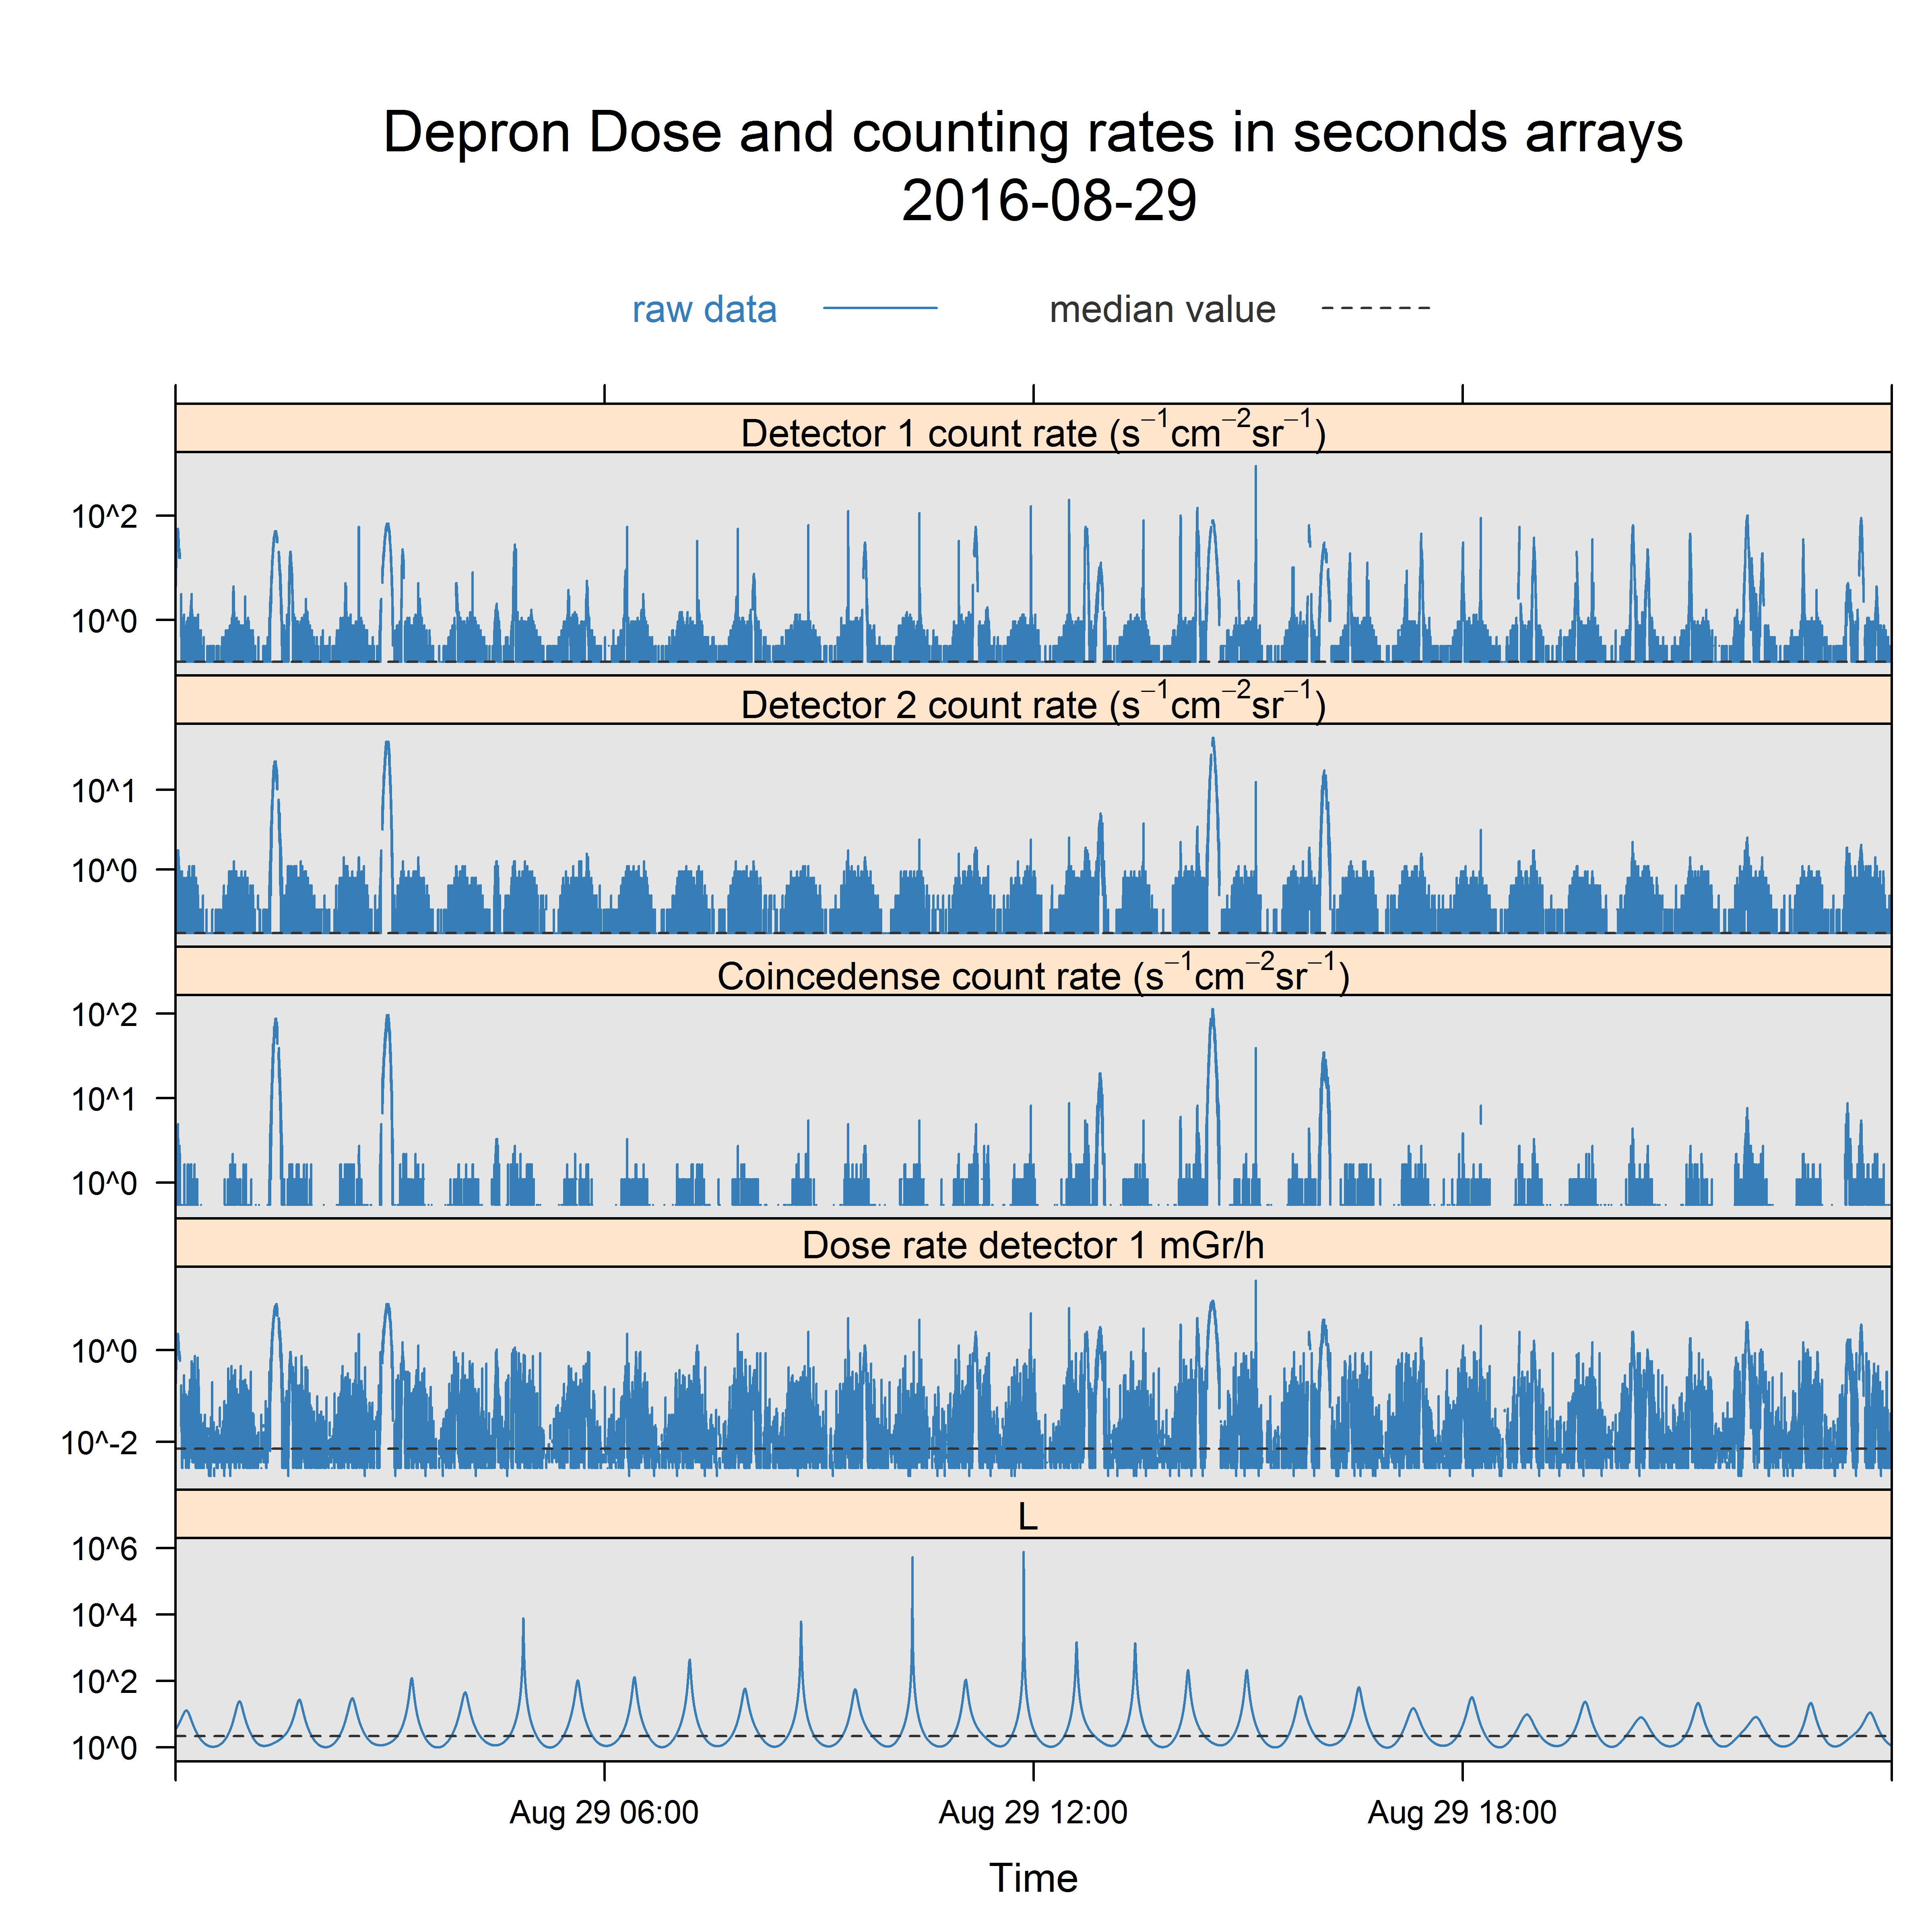
\includegraphics[width=0.5\linewidth]{images/results/depron_sec_log08-29-16}
	\caption{Временные серии  измерений детекторов прибора ДЭПРОН. }
	\label{fig:depronseclog08-29-16}
\end{figure}
Так как секундные данные содержат существенный разброс значений из-за малой статистики отсчетов, был предложен и реализован алгоритм треугольного сглаживания, который позволяет выявлять только значимые изменения в исходных данных. Пример использования этого алгоритма показан на рисунке 	\ref{fig:depronseclognew08-29-16}.
\begin{figure}
	\centering
	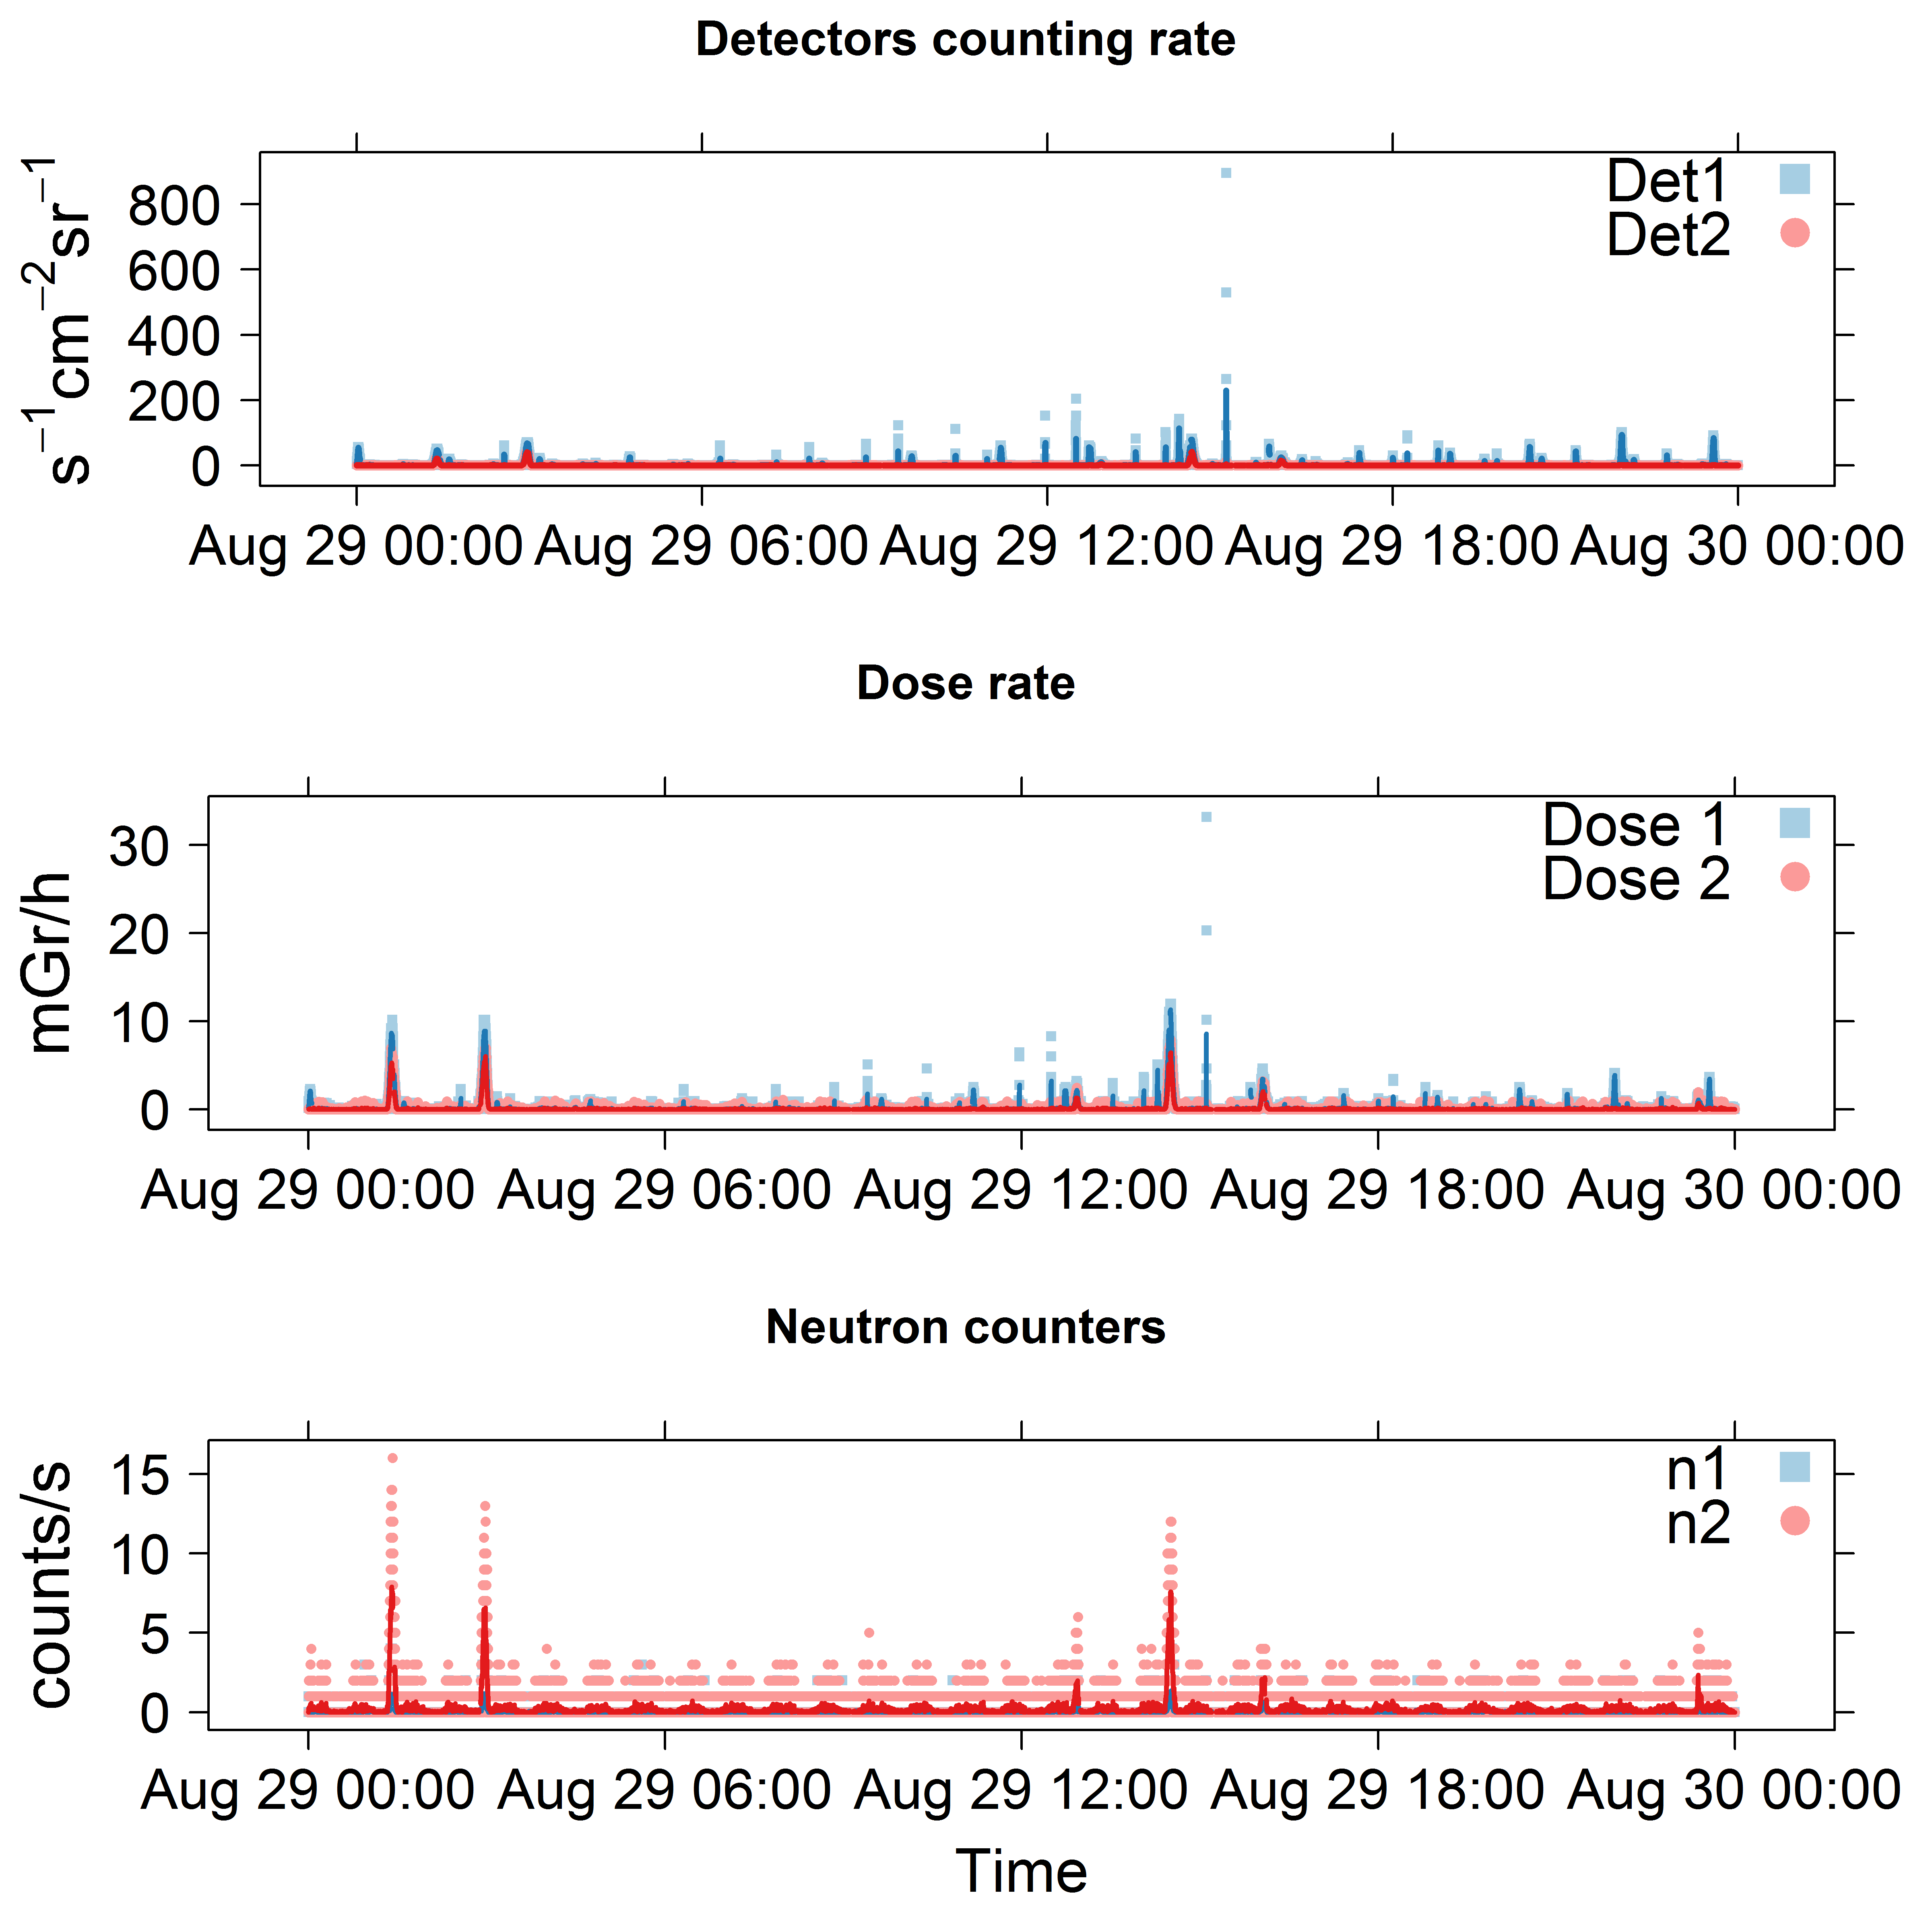
\includegraphics[width=0.5\linewidth]{images/results/depron_sec_log_new08-29-16}
	\caption{Временные серии измерений ДЭПРОН со сглаживанием. }
	\label{fig:depronseclognew08-29-16}
\end{figure}
В первую очередь для каждого дня работы прибора были построены карты скоростей счета в первом детекторе \ref{sec:planetDose}.В процессе построения пространственного распределения было обнаружено расхождение меток времени  ДЭПРОН и всемирного времени. Разработанное решение проблемы привязки данных подробно рассматривается в разделе \ref{sec3.2}.

Аналогично картам, были построены долготные зависимости скоростей счета в первом детекторе, эти графики позволили оперативно заметить резкие всплески потоков частиц во внешнем радиационном поясе \label{sec:flash_analisys}. Также для каждого дня были построены карты скоростей счета в координатах Мак-Илвайна \cite{McIlwain1961}, которые были рассчитанны по модели IGRF.

\section{Планетарное распределение потоков частиц, мощности дозы на высоте полета КА а также потоков нейтронов} \label{sec:planetDose}
При последующей обработке данных были построены графики географического распределения скоростей счета во всех детекторах прибора - двух полупроводниковых и двух нейтронных счетчиков. Цветовая схема для карт подобрана таким образом, чтобы максимальные значения были отображены красным цветом а минимальные синим, между конечными точками цвет изменяется по градиенту. Цветовая палитра квантована на 20 дискретных цветов. Каждому значению полученной дозы ставится в соответствие индекс в массиве цветов, который вычисляется по формуле:
\begin{equation*}
index_{color} = \begin{cases}
	8*\log{10}(N + 1)+1,  & \text{если } 8*\log{10}(N + 1) +1 < n \\
	n,  & \text{если } 8*\log{10}(N + 1) +1 \ge n
	\end{cases}
\end{equation*}
		где $ n $ -- цветность палитры, а $ N $ -- величина, подлежащая отображению.
						
% col = colr[ifelse(ceiling(8*log10(as.integer(combined.zoom$count1)+1))+1>n,
%n,
%ceiling(8*log10(as.integer(combined.zoom$count1)+1))+1)]
%
На картах 	\ref{fig:depronmap241} каждый маркер представляет результаты измерений детекторов за одну секунду. В качестве маркера выбран незакрашенный круг, так как в отличие от точки или линии он позволяет покрыть некоторую площадь на графике. Размер маркера подобран исходя из соображений заметания определенной площади, так как  при полете по орбите спутник покрывает 7,5 км каждую секунду. Маркеры частично перекрываются, особенно в полярных областях и наилучшие результаты по отображению были получены при использовании частичной прозрачности. Для простоты отображения выбрана прямоугольная проекция карты по широте и долготе, поэтому на различных широтах площадь отображаемой поверхности не искажена. Это обстоятельство таким образом лишь условно соотвествует величине траектории вдоль которой производилось измерение.
\begin{figure}[h]
	\centering
	\includegraphics[width=0.7\linewidth]{images/depronmap241}
	\caption{Карта распределения счета в первом детекторе.}
	\label{fig:depronmap241}
\end{figure}

\section{Распределение мощности дозы вне радиационных поясов Земли}
Данные за все время измерений были разделены на зоны соответствующие участкам траектории, проходящим через ЮАА, внешний радиационный пояс, а также всем оставшимся участкам траектории спутника. Разделение было проведено по геомагнитным координатам. 
\begin{verbatim}
combined.zoom.anom<-filter(combined, b<0.21)
combined.zoom.polar <-filter(combined,l<7,l>3)
combined.zoom.regular<-filter(combined,l>7|l<3,b>0.21)
\end{verbatim}
Разделение по геомагнитным координатам позволило для большинства дней отделить высокие по величине вклады ЮАА и авроральных областей, оставшиеся части траектории несут радиационную нагрузку, показанную на рисунке \ref{fig:gcrdose}. 
\begin{figure}
	\centering
	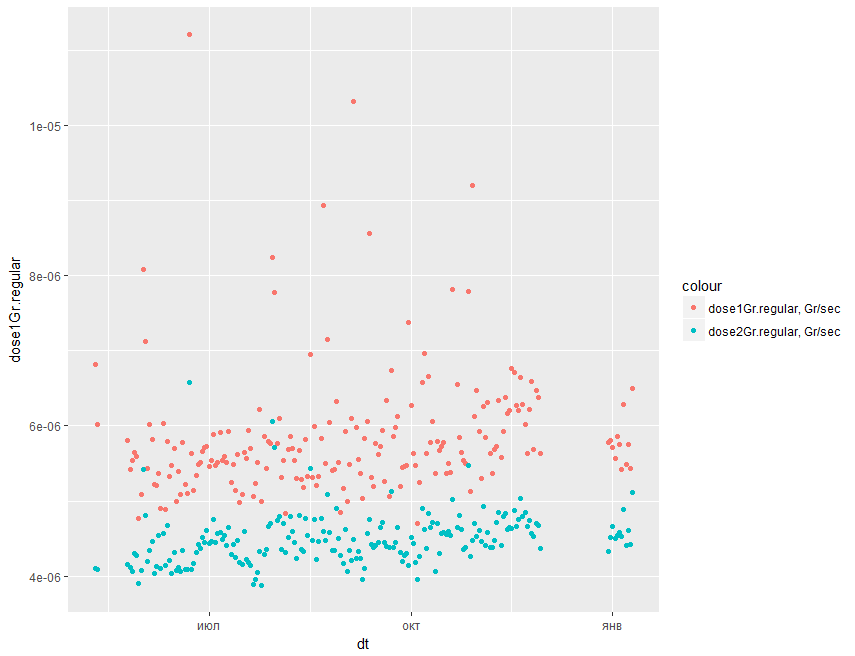
\includegraphics[width=0.5\linewidth]{images/doseanalisys/GCRdose}
	\caption{Поглощенные дозы за сутки, полученные при полете спутника вне ЮАА и внешнего радиационного пояса. Основной вклад в дозу вносит ГКЛ.}
	\label{fig:gcrdose}
\end{figure}
Основной вклад в поглощенную дозу в этих зонах вносит ГКЛ, которое слабо моделируется солнечной активностью и на протяжении годового цикла измерений в 2016 году меняется незначительно, этот факт подтверждается надежными измерениями сети наземных нейтронных мониторов \ref{fig:nmdb2016}. Тем не менее, на выделенных зонах видно несколько выбросов до величин мощности дозы в 10\textsuperscript{-4} Гр/с. Эти выбросы свидетельствуют, что разделение по геомагнитным координатам не позволяет полностью отделять авроральную зону и ЮАА. Причина вероятно заключается в возмущенной геомагнитной обстановке в эти периоды времени, она приводит к смещению реальных значений B и L, относительно расчетных по модели IGRF, которые были использованы при привязке данных ДЭПРОН.

\begin{figure}
	\centering
	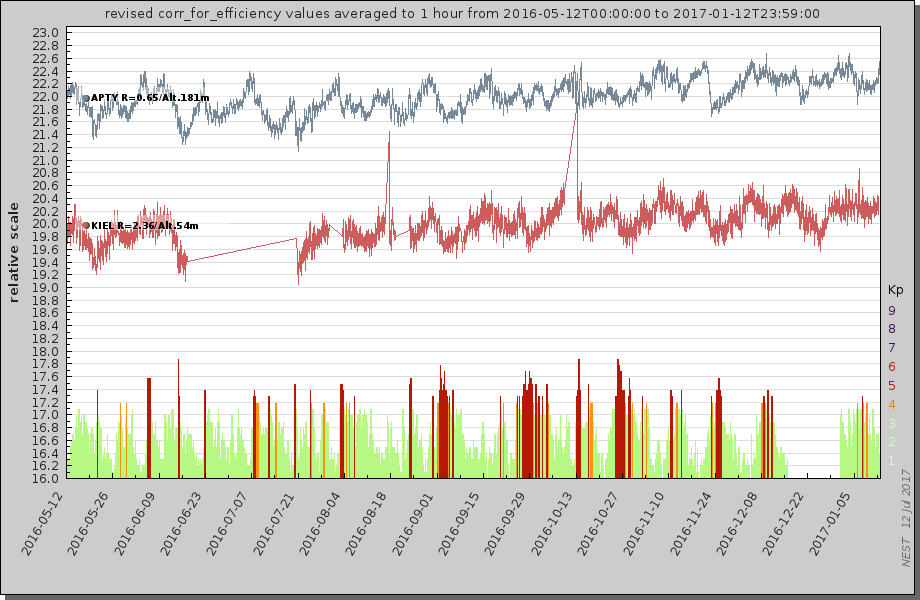
\includegraphics[width=0.7\linewidth]{images/nmdb2016}
	\caption{Данные нейтронным мониторов за период работы прибора ДЭПРОН в 2016-207 гг. По материалам из базы данных \href{www.nmdb.eu}{NMDB}, основанную в рамках программы Европейского союза FP7 (контракт № 213007) для предоставления данных \cite{Ibragimov}. Верхняя кривая представляет данные нейтронного монитора в Апатитах, нижняя кривая представляет данные монитора в Киль, Германия. Измерения представлены в относительных единицах, нормированных на атмосферное давление и эффективность регистрации.}
	\label{fig:nmdb2016}
\end{figure}

\section{Распределения мощности дозы в области ЮАА}
Из результатов исследований НИИЯФ МГУ \cite{Lishnevskii2012} известно, что дозы,  набираемые при пролетах МКС через области аномалии являются значительными несмотря на малые участки траектории пересекающие аномалию. Аналогичная ситуация возникает и на высокоширотной полярной орбите, это подтверждают данные ДЭПРОН, так как он работает на полярном аппарате Ломоносов. 

В качестве примера возьмем временные серии скоростей счета и мощности дозы, полученные с ДЭПРОН для 14:30 29 Августа 2016 года \ref{fig:depronseclognew08-29-1614-24-23}. Возрастание скоростей счета и доз связано с пересечением ЮАА. Точками показаны измерения с детекторов с секундным разрешением, сплошными линиями отражено сглаживание данных треугольным фильтром.

\begin{figure}
	\centering
	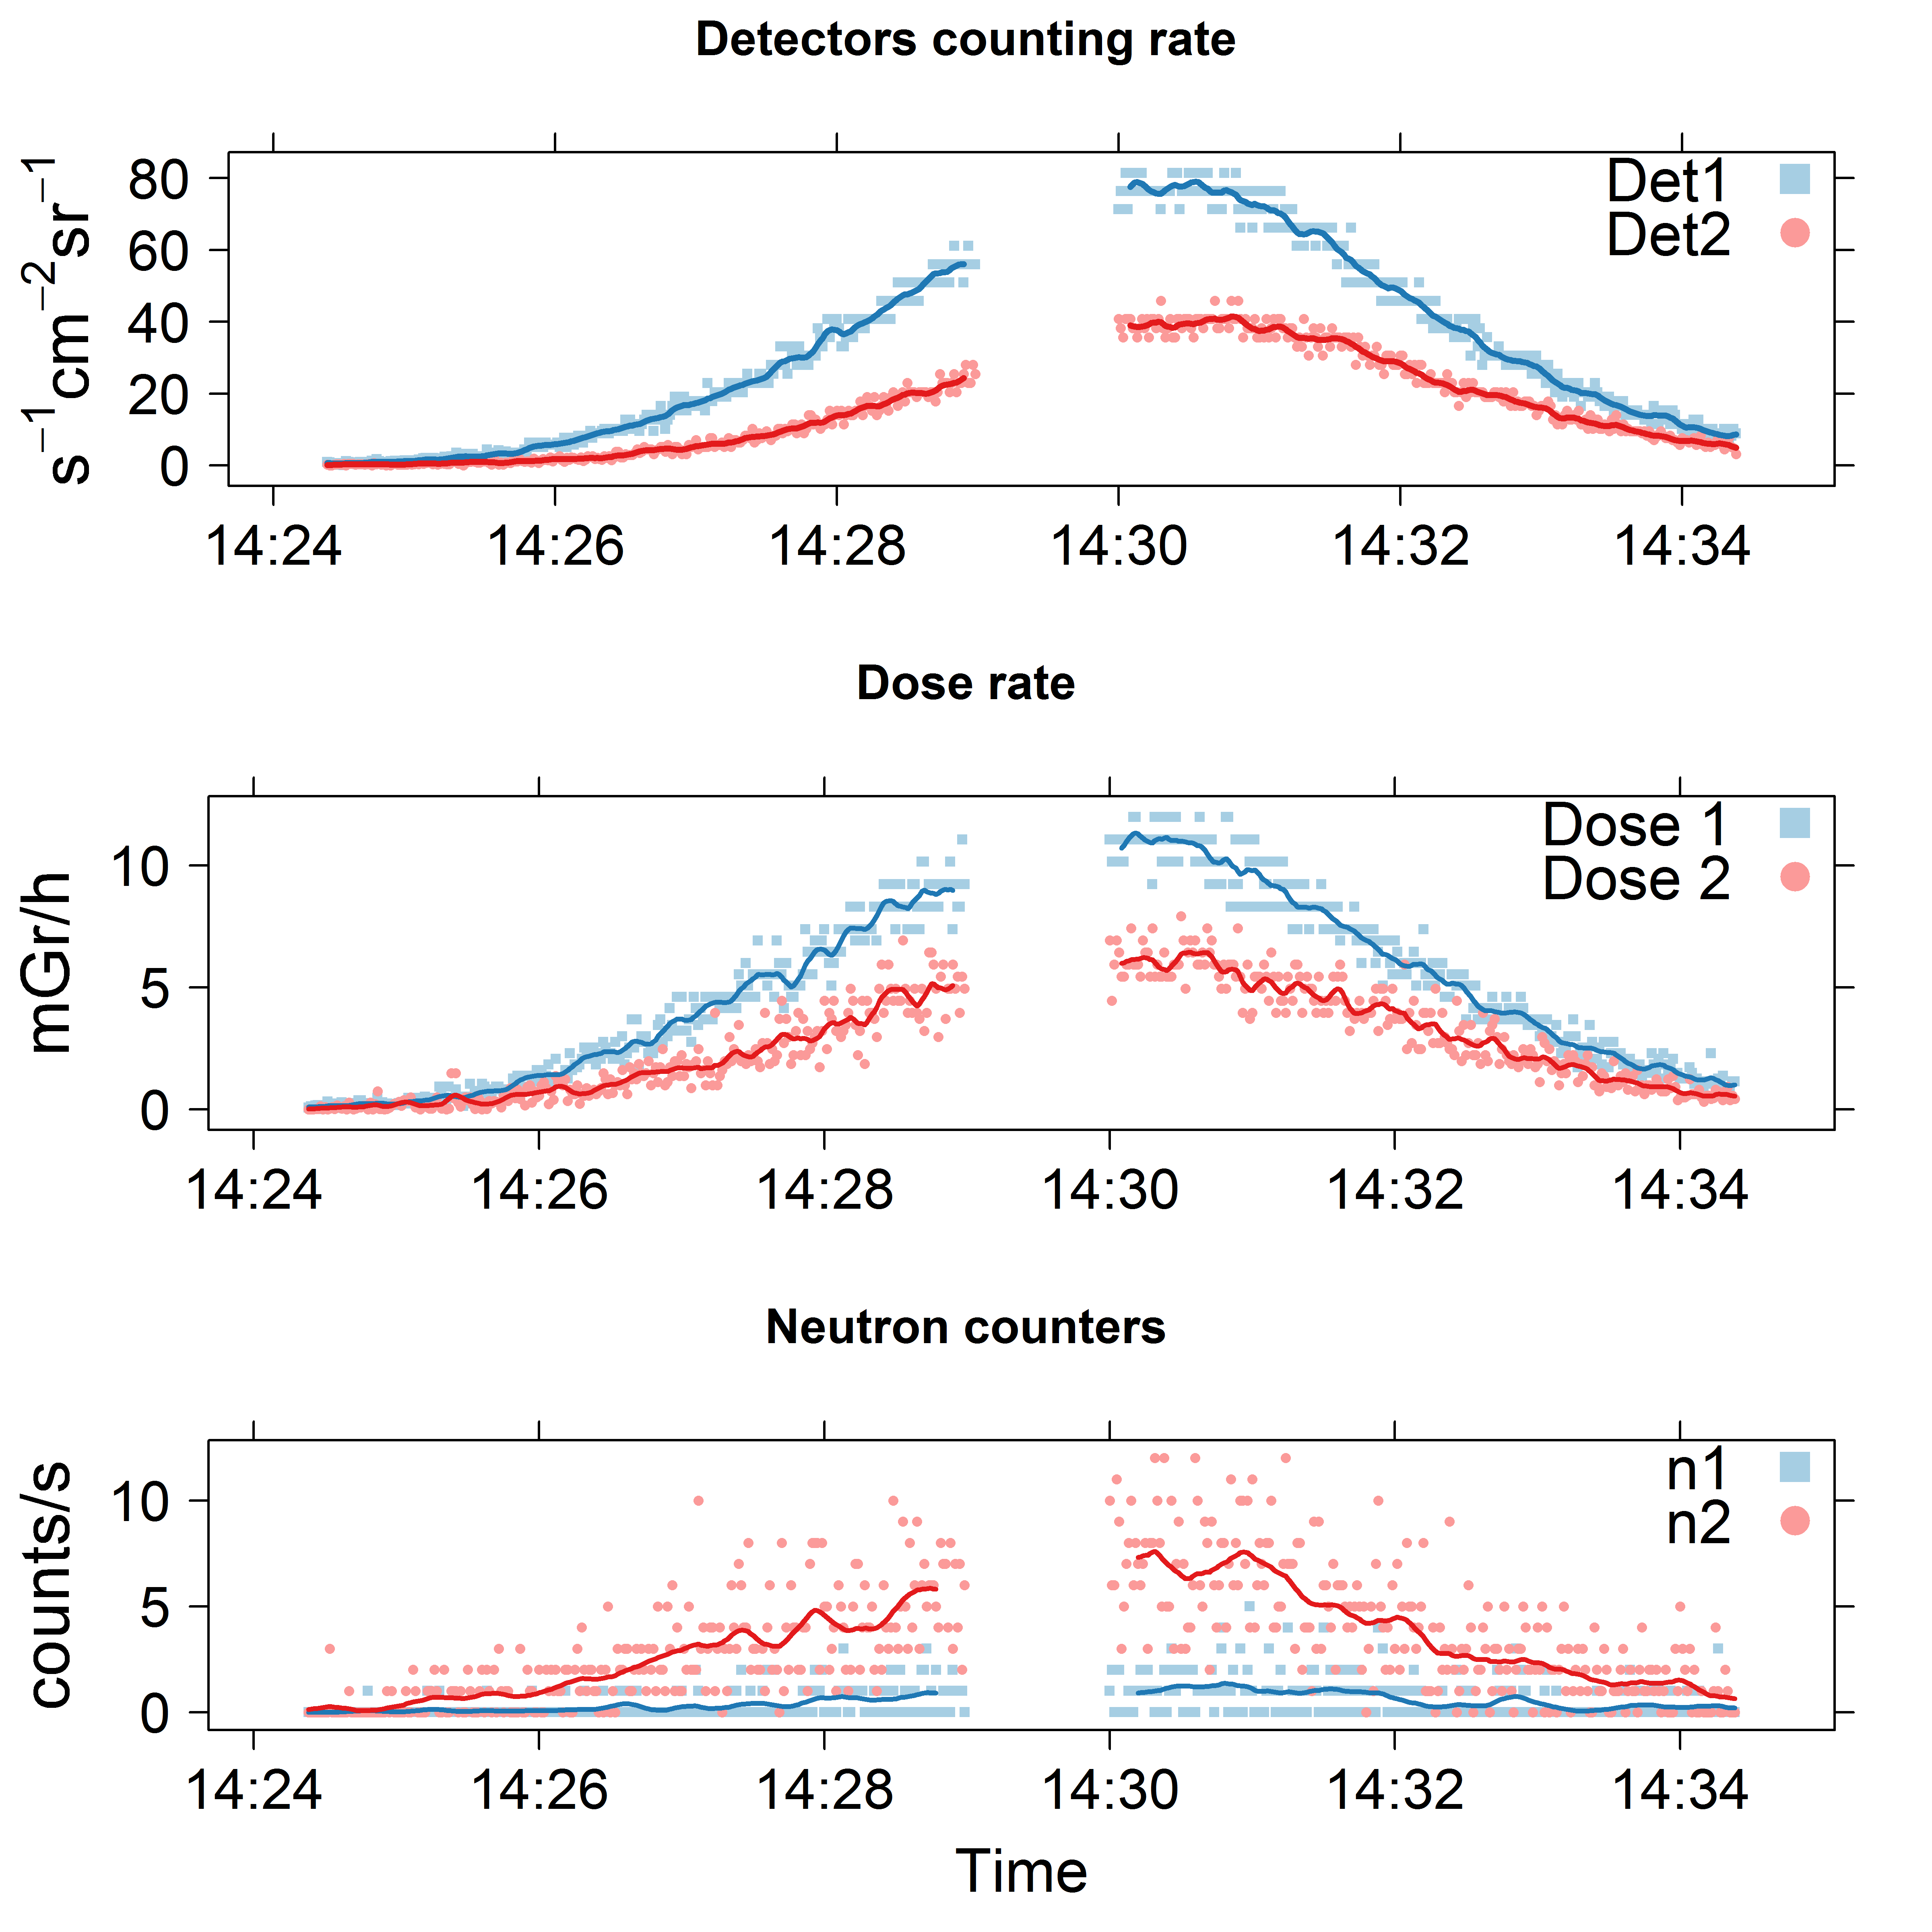
\includegraphics[width=0.5\linewidth]{images/results/depron_sec_log_new08-29-1614-24-23}
	\caption{Временные серии скоростей счета и мощности дозы при пересечении внутреннего радиационного пояса}	\label{fig:depronseclognew08-29-1614-24-23}
\end{figure}

Видно, что в данных отсутствует минута измерений 14:29, это является последствием загруженности канала передачи данных. Также можно наблюдать, что верхний полупроводниковый детектор показывает потоки в два раза превышающие потоки во втором детекторе. Причем, важно отметить, что эти значения уже нормированы на геометрический фактор и представляют собой истинные интегральные потоки для заряженных частиц, различающиеся только нижней границей энергии регистрации. Подробнее границы энергетической чувствительности обсуждаются в разделе \ref{sec:energy}.

Аналогично потокам частиц, поглощенные дозы в аномалии относятся с фактором 2. Совпадение  величины отношения дозы и отношения счета частиц в двух детекторах показывает, что в зоне ЮАА половина частиц проникает через оба детектора и теряет незначительную долю энергии при прохождении через верхний детектор и разделяющие детекторы слои вещества в приборе. Те же частицы, которые не долетают до второго детектора имеют близкие энергетические характеристики, так как они вносят вклад в дозу прямо пропорциональный их потоку. Причиной такого характера работы полупроводниковых детекторов может являться более высокий порог регистрации у второго детектора по сравнению с первым детектором.

Счет в нейтронных счетчиках отличается более значительно, показания более защищенного детектора от 2 до 4 раз выше чем менее защищенного. Это 




\section{Распределения мощности дозы в авроральных областях}


Также построены зависимости скорости счета от времени и параметра L \ref{fig:l-t2016}а. Для сравнения представлены результаты измерений электронов с энергиями более 2 МэВ на спутниках Van Allen \ref{fig:van-allen-lshell-crop}б. 

\def\imagetop#1{\vtop{\null\hbox{#1}}}
\begin{figure}
%	\centering
	\begin{tabular}{l l}
		\imagetop{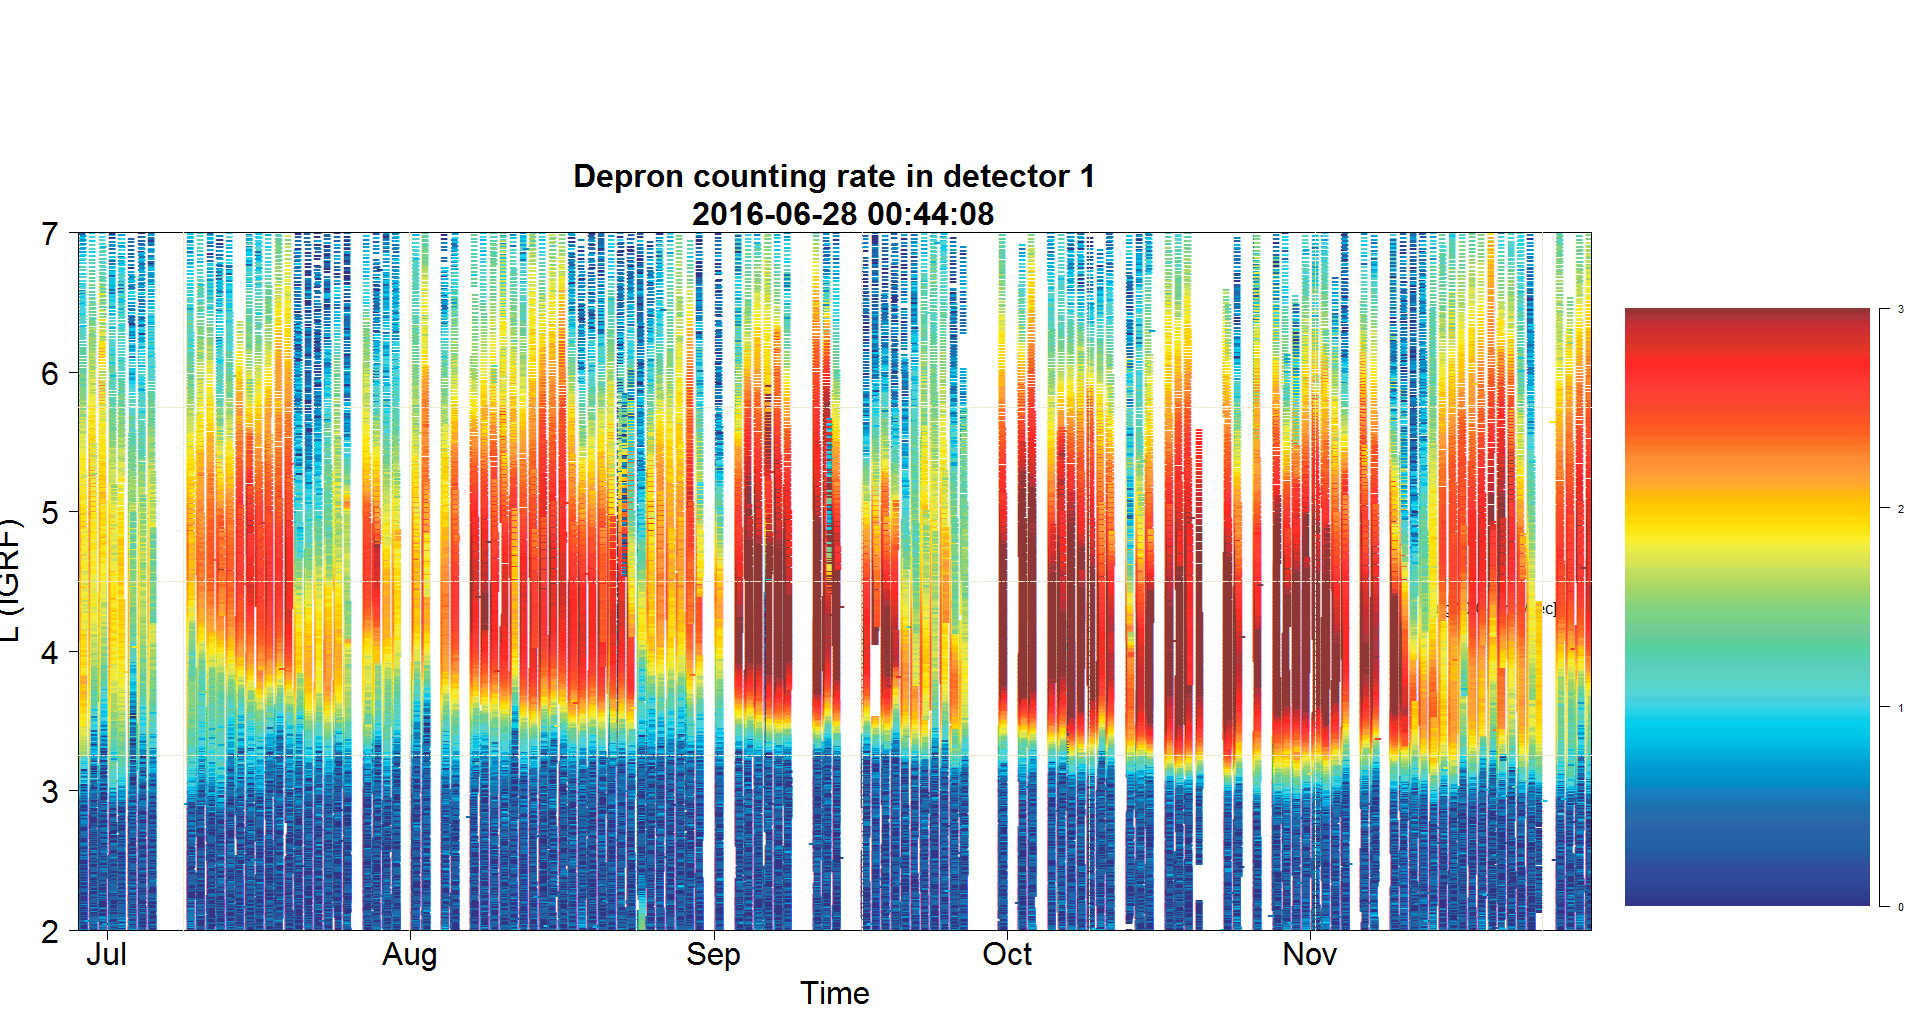
\includegraphics[width=0.9\linewidth]{images/L-t2016}} & \imagetop{(а)} \\
		\imagetop{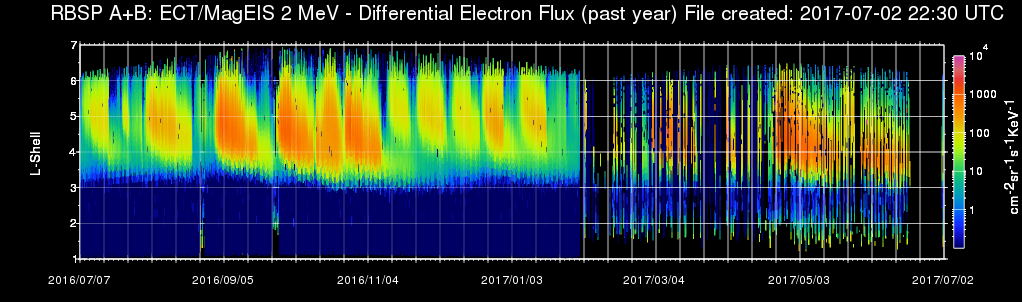
\includegraphics[width=0.9\linewidth]{../literature_repository/relelec/van-allen-lshell-crop-box}} & \imagetop{(б)}
	\end{tabular}
	\caption{а. Зависимость скорости счета в первом детекторе от времени и параметра Мак-Илвайна L.\\ б. Дифференциальный поток электронов с энергией более 2 МэВ, по данным спутников RPSB A и RPSB B. По материалам: \cite{NOAA}.}
	
	\label{fig:l-t2016}
\end{figure}


\section{Анализ возрастаний потоков частиц в областях внешнего радиационного пояса}\label{sec:flash_analisys}
В  данных  ДЭПРОН приполярные области отличаются высокой вариабельностью во времени и пространстве потоков частиц и соответственно доз. Были найдены и выделены возрастания скоростей счета в первом детекторе	\label{fig:depronlatmap148}, превышающие по абсолютной величине 5000 отсчетов в секунду, что соответствует более 800 с\textsuperscript{-1} см\textsuperscript{-1} стер\textsuperscript{-1}. 
\begin{figure}[h]
	\centering
	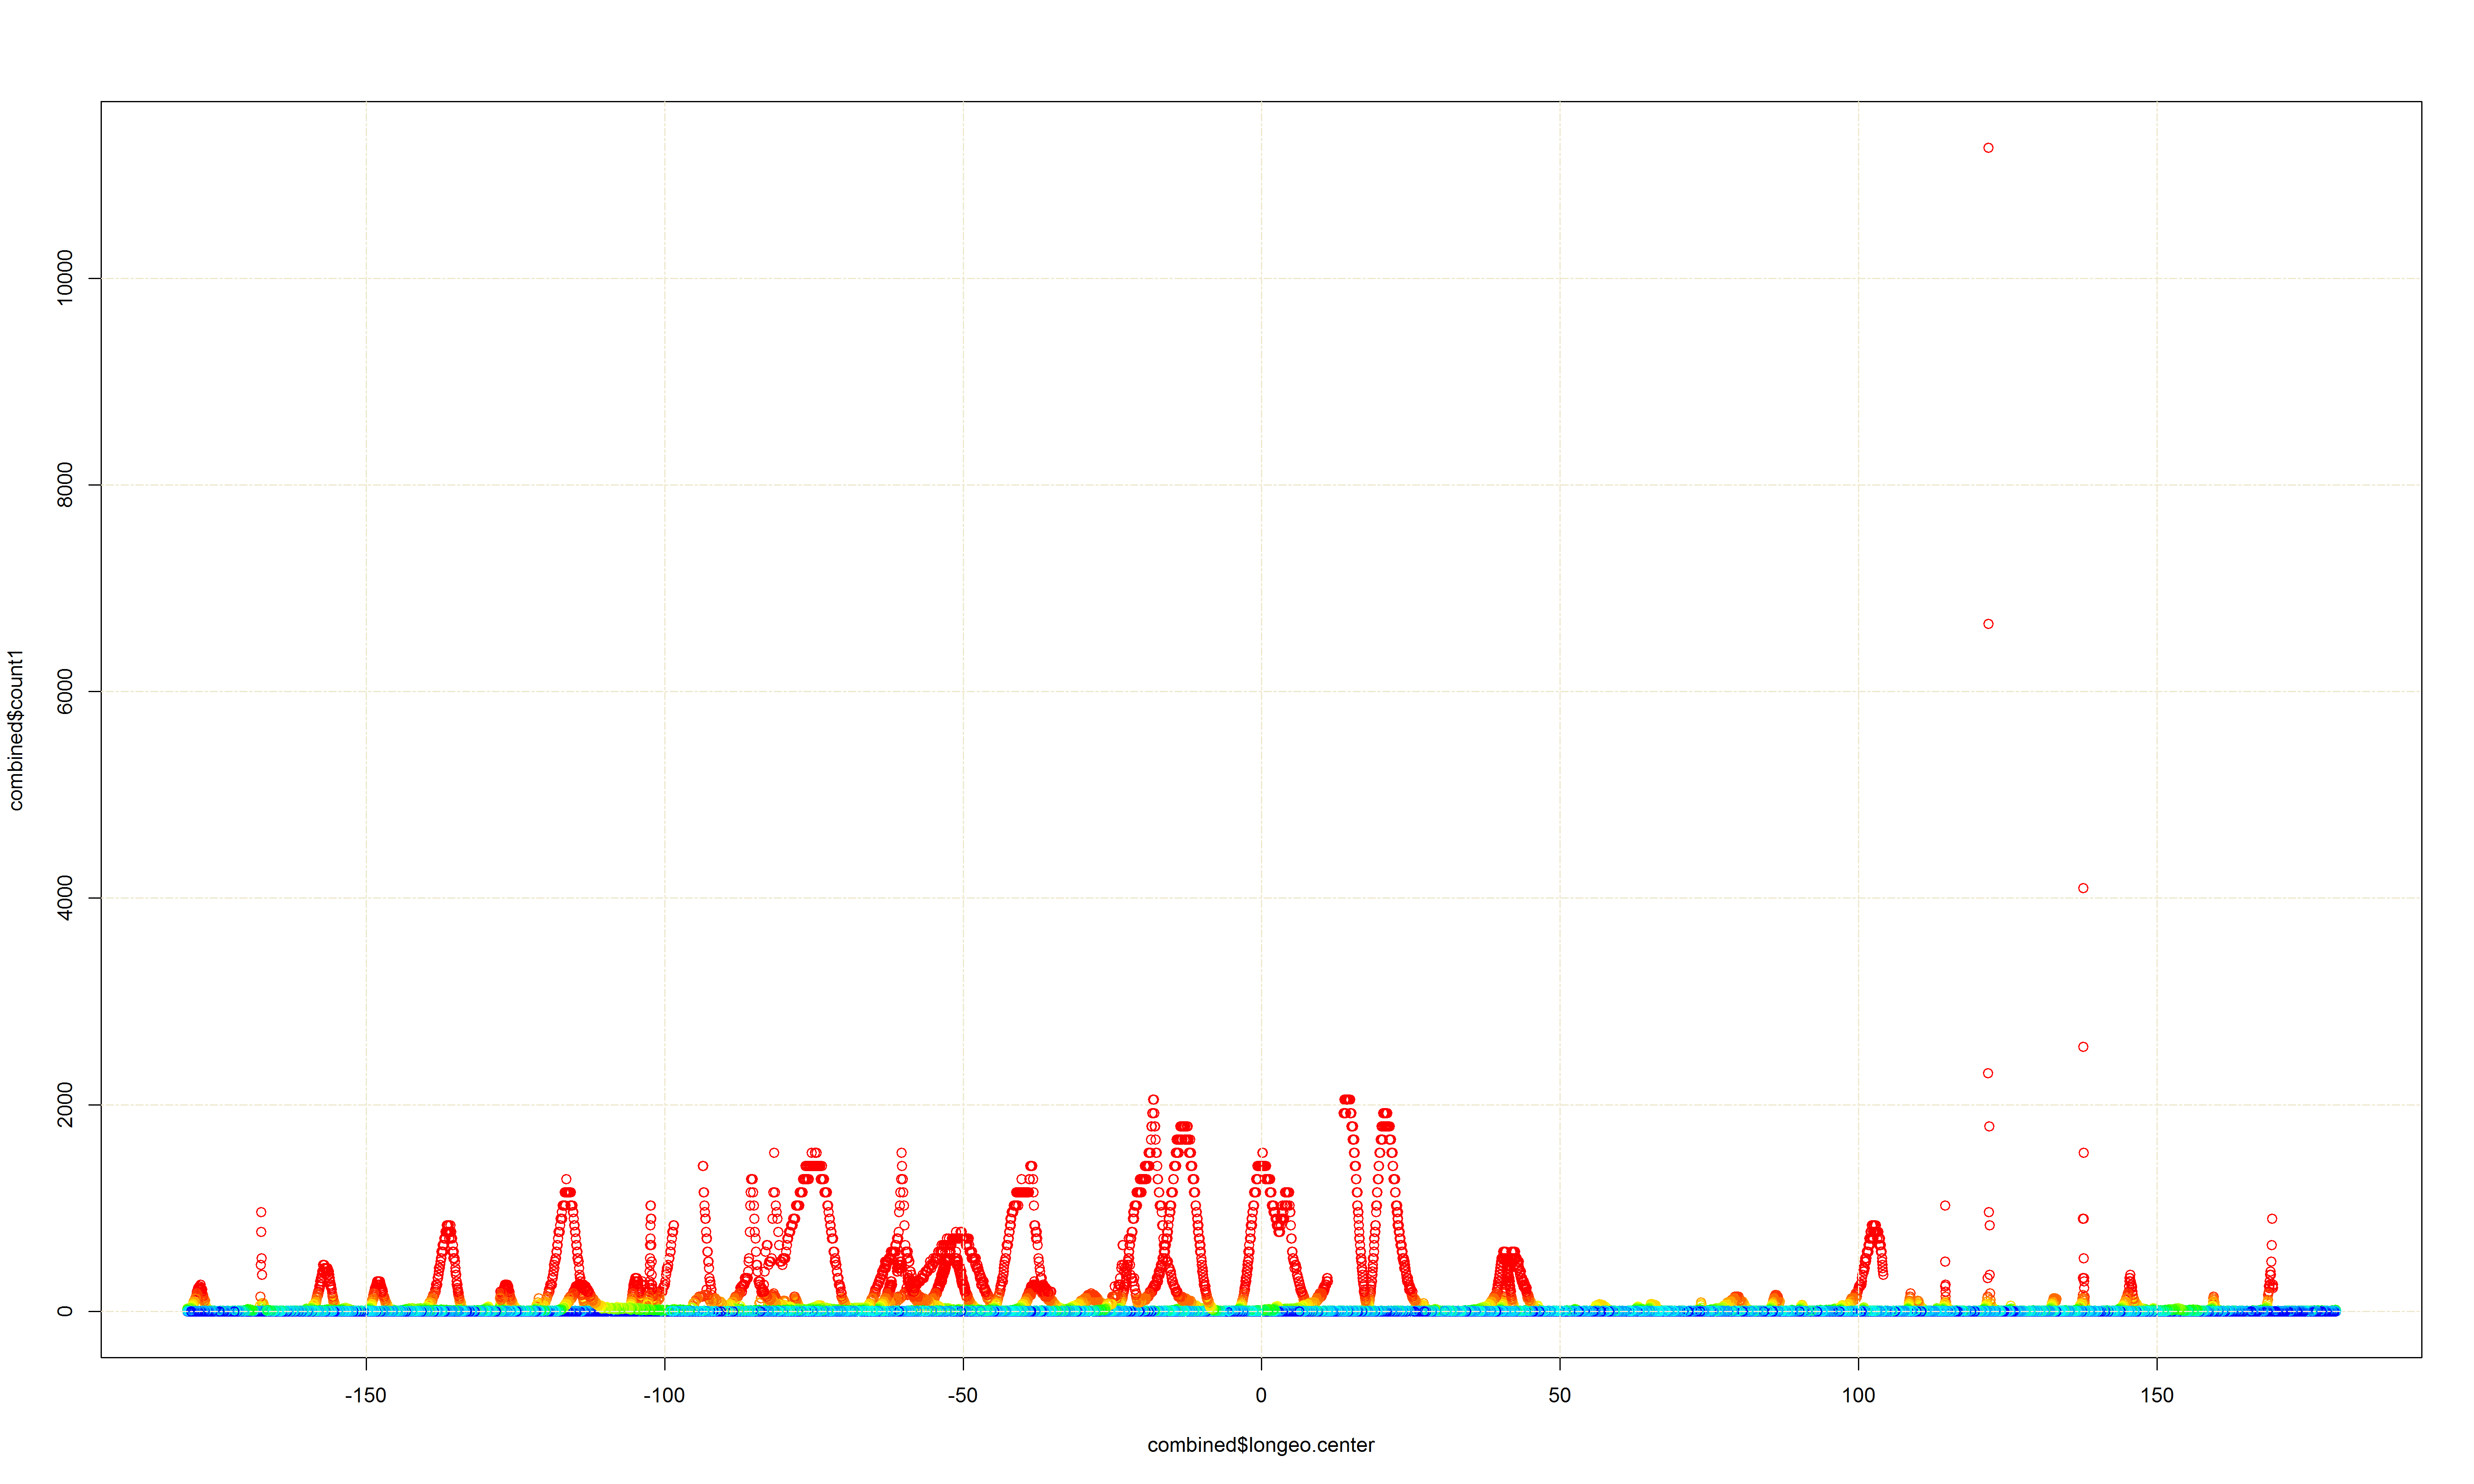
\includegraphics[width=0.8\linewidth]{images/Flash/depron_lat_map_148}
	\caption{Географическое распределение потоков заряженных частиц в первом полупроводниковом детекторе. Для наглядности счет в детекторе показан в линейном масштабе.}
	\label{fig:depronlatmap148}
\end{figure}
Величины повышенных потоков, зарегистрированных в первом полупроводниковом детекторе в среднем в 30-100 раз выше чем во втором детекторе и при одновременной регистрации в двух детекторах.
\begin{figure}[h]
	\centering
	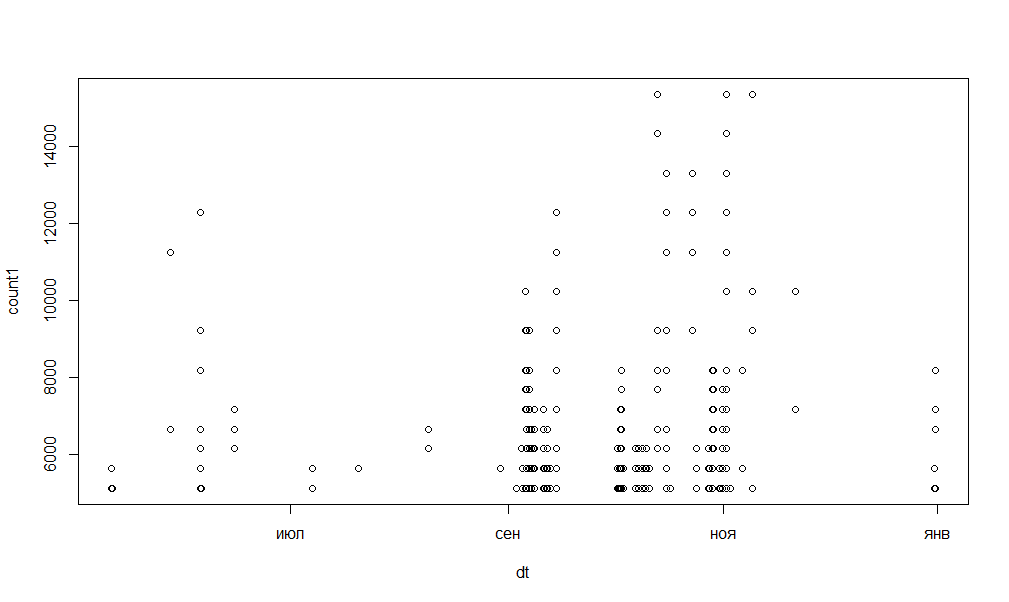
\includegraphics[width=0.7\linewidth]{images/Flash/Rplot03}
	\caption{Временное распределение зарегистрированных вспышек. Общее число выделенных вспышек за время работы прибора ДЭПРОН достигает 90.}
	\label{fig:rplot03}
\end{figure}

Учитывая, что геометрический фактор телескопа детекторов в 3 раза меньше чем геометрический фактор верхнего детектора, мы можем предположить что энергии частиц в этих потоках невысоки, поэтому большая часть частиц до второго детектора не доходит.	Для наибольших возрастаний счета отношение скоростей счета меньше и составляет один порядок и здесь энергия частиц больше. Мы наблюдаем четкое разделение по скорости счета и соотношению в верхнем и нижнем детекторах. 
\begin{figure}[h]
	\centering
	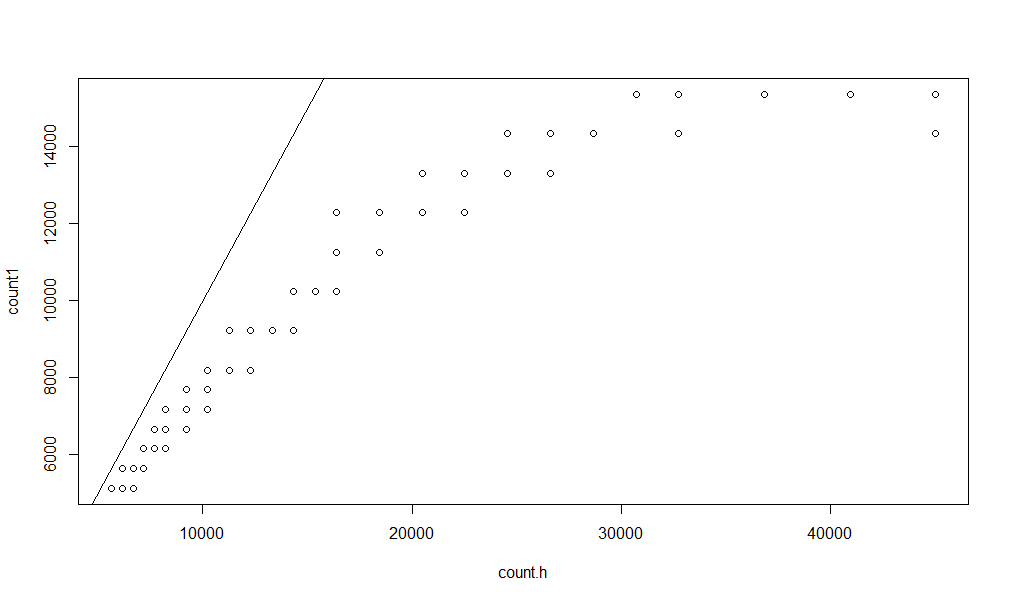
\includegraphics[width=0.7\linewidth]{images/Flash/Rplot04}
	\caption{Соотношение программного и аппаратного счетчиков для моментов времени, в которые регистрировались вспышки. Прямая на рисунке показывает соотношение при котором все зарегистрированные частицы обработаны программой прибора. Каждая точка показывает интегральный счет за одну секунду.}
	\label{fig:rplot04}
\end{figure}
Соотношение аппаратного счетчика первого детектора и программного счетчика позволяет сделать вывод, что при высоких загрузках микроконтроллер ДЭПРОН не успевает программно обработать все зарегистрированные детекторами частицы. Зависимость \ref{fig:rplot04} отношения обработанных и всех частиц практически линейна до скоростей счета 5000 за секунду, а более 10 тысяч отсчетов становиться нелинейной. Поэтому в максимальных импульсах, зарегистрированных за время работы ДЭПРОН, не было обработано в три раза больше прерываний от частиц, по сравнению с числом обработанных программных прерываний. Это обстоятельство позволяет сделать поправки в большую сторону при оценке дозовых нагрузок во время вспышек. 

Для анализа различных параметров возрастаний были построены матричные графики всех доступных переменных друг относительно друга 	\ref{fig:rplot08}. Можно заметить, что параметр L меняется в пределах от 3 до 5,5. При этом максимальные величины потоков были зарегистрированы на L оболочке равной четырем. Значения напряженности магнитного поля B находятся в пределах от 0,26 до 0,5 Гн. Максимальные потоки были зарегистрированы при B около 0,35 Гн. 

Нейтронные счетчики в моменты регистрации вспышек не показывают какого-либо увеличения счета. Максимальные значения 2-3 отсчета в секунду, а средние величины менее 1 нейтронов за 5 секунд, они являются нормальными для данных широт.

Были рассмотрены зависимости дозы в L-B координатах, о наличии магнитной бури следить по индексам A(e) A(l), причем по мнению Антоновой стоит выбрать спокойный период. с разделением утреннее в вечернего местное магнитное время (MLT) 

\begin{figure}
	\centering
	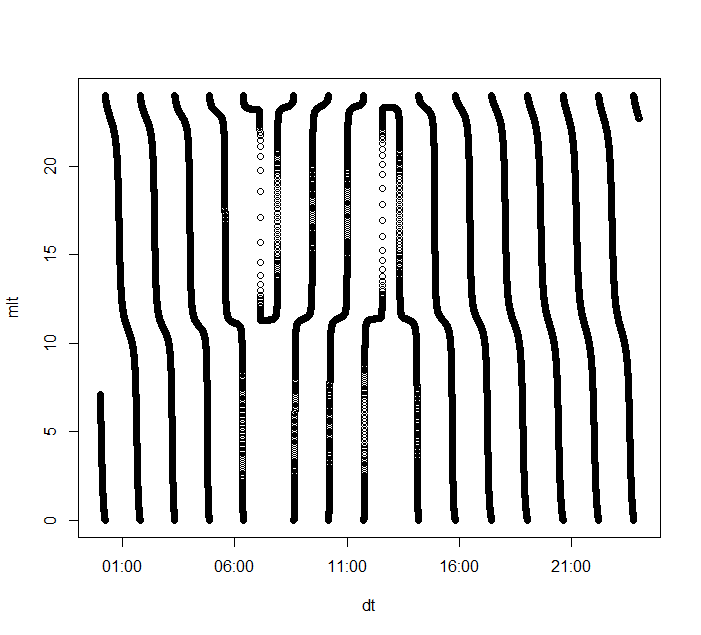
\includegraphics[width=0.49\linewidth]{images/Flash/Rplot15}
	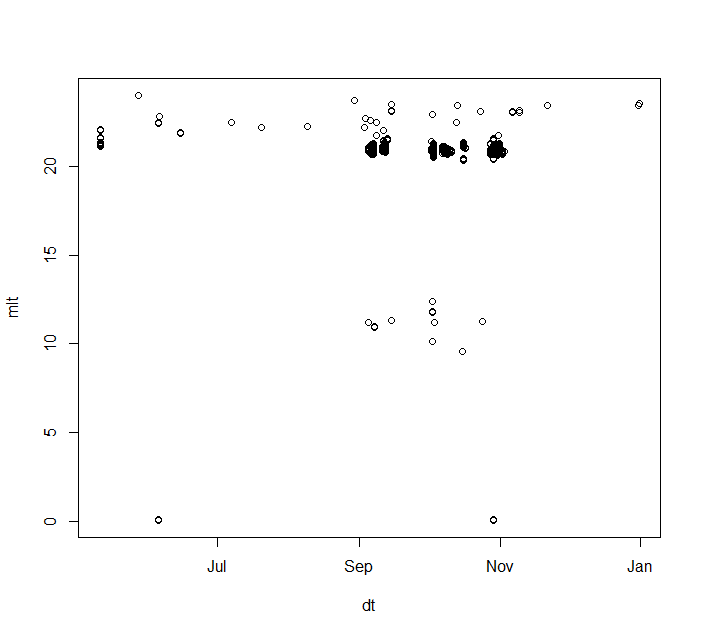
\includegraphics[width=0.49\linewidth]{images/Flash/Rplot14}
	\caption{Магнитное локальное время для зарегистрированных }
	\label{fig:rplot15}
\end{figure}


%Построены зависимости B(t) для L из диапазонов от 4-5, 5-6, 6-7.




%\section{Спектры ЛПЭ и распределение мощности эквивалентной дозы}